  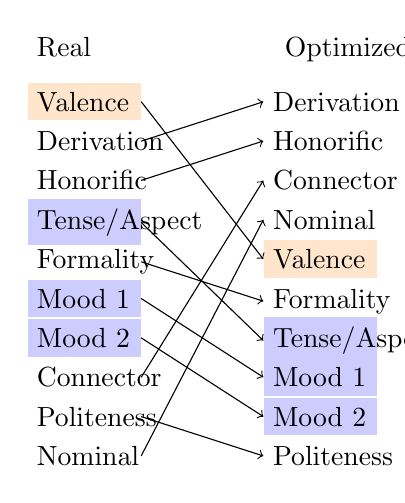
\begin{tikzpicture}[%
% common options for blocks:
block/.style = {draw, fill=blue!30, align=center, anchor=west,
            minimum height=0.65cm, inner sep=0},
% common options for the circles:
ball/.style = {circle, draw, align=center, anchor=north, inner sep=0}]
\node[rectangle,text width=1.2cm,anchor=base] (A0) at (1,-0.3) {Real};
\node[rectangle,text width=0.9cm,anchor=base] (B0) at (4,-0.3) {Optimized};
\node[rectangle,text width=1.2cm,anchor=base, fill=orange!20] (A1) at (1,-1.0) {Valence};
\node[rectangle,text width=1.2cm,anchor=base] (A2) at (1,-1.5) {Derivation};
\node[rectangle,text width=1.2cm,anchor=base] (A3) at (1,-2.0) {Honorific};
\node[rectangle,text width=1.2cm,anchor=base, fill=blue!20] (A4) at (1,-2.5) {Tense/Aspect};
\node[rectangle,text width=1.2cm,anchor=base] (A5) at (1,-3.0) {Formality};
\node[rectangle,text width=1.2cm,anchor=base, fill=blue!20] (A6) at (1,-3.5) {Mood 1};
\node[rectangle,text width=1.2cm,anchor=base, fill=blue!20] (A7) at (1,-4.0) {Mood 2};
\node[rectangle,text width=1.2cm,anchor=base] (A8) at (1,-4.5) {Connector};
\node[rectangle,text width=1.2cm,anchor=base] (A9) at (1,-5.0) {Politeness};
\node[rectangle,text width=1.2cm,anchor=base] (A10) at (1,-5.5) {Nominal};
\node[rectangle,text width=1.2cm,anchor=base] (B1) at (4,-1.0) {Derivation};
\node[rectangle,text width=1.2cm,anchor=base] (B2) at (4,-1.5) {Honorific};
\node[rectangle,text width=1.2cm,anchor=base] (B3) at (4,-2.0) {Connector};
\node[rectangle,text width=1.2cm,anchor=base] (B4) at (4,-2.5) {Nominal};
\node[rectangle,text width=1.2cm,anchor=base, fill=orange!20] (B5) at (4,-3.0) {Valence};
\node[rectangle,text width=1.2cm,anchor=base] (B6) at (4,-3.5) {Formality};
\node[rectangle,text width=1.2cm,anchor=base, fill=blue!20] (B7) at (4,-4.0) {Tense/Aspect};
\node[rectangle,text width=1.2cm,anchor=base, fill=blue!20] (B8) at (4,-4.5) {Mood 1};
\node[rectangle,text width=1.2cm,anchor=base, fill=blue!20] (B9) at (4,-5.0) {Mood 2};
\node[rectangle,text width=1.2cm,anchor=base] (B10) at (4,-5.5) {Politeness};
\draw[->] (A1.east) to (B5.west);
\draw[->] (A2.east) to (B1.west);
\draw[->] (A3.east) to (B2.west);
\draw[->] (A4.east) to (B7.west);
\draw[->] (A5.east) to (B6.west);
\draw[->] (A6.east) to (B8.west);
\draw[->] (A7.east) to (B9.west);
\draw[->] (A8.east) to (B3.west);
\draw[->] (A9.east) to (B10.west);
\draw[->] (A10.east) to (B4.west);
\end{tikzpicture}
